% Chapter 3

\chapter{A self regulation approach} % Main chapter title

\label{Chapter3} % For referencing the chapter elsewhere, use \ref{Chapter1}

We started working on our system as a solution for parents who wanted a reliable parental control system, which tries to use the newest discoveries related to parental control impact on child development and is also easy to install and use. Most of the existing parental control systems are subscription based and work by creating a custom configuration for a specific family and enforcing the rules by using a client application for each target device. We wanted to design our system such that the user is in full control of the system configuration and all the data is kept locally, because we saw no point in getting the data outside the house, since its only use is only inside the local network, at least for out system. The system that we developed does not require any kind of client configuration, all the configuration needed is done on the central node, which in out case is a Raspberry Pi, which is an access point and a system control node, and a mobile application which the parents use to configure the parental control policies. We also offer a client application design for children devices, but that is only to extend the basic functionality and to also help with some initial configuration. So we basically moved the configuration part from the clients to the central node of the system. We tried to make the configuration as simple as possible, such that even a non-technical person can configure and start the system. The only commercial level alternative control parental system that we found using the same approach is Circle With Disney, whose details we presented in \ref{Chapter2}. It uses an additional network device which you have to purchase and it work by connecting to the local wireless network and using a technique called ARP Spoofing, used mostly for network attacks, because it aims to associate and attacker's MAC address with the IP address of another host, such as the default gateway, causing any traffic meant for that IP address to be sent to the attacker instead. Because we are building out system around the access point, instead of using an additional device, we have much more flexibility in the techniques we use for filtering and blocking at potentially a higher cost for the device. Any type of network device with a wireless card can be used to establish this kind of setup, but we used a Raspberry Pi because it is a cheap device, having almost the same price as a good router, and is quite powerful and flexible. Another difference between out approach and the Circle device is that the core of system is built around the  Domain Name System, by using a local DNS server for filtering and blocking. For this test we are using the open source project Pi-hole, which uses the DNS forwarder and DHCP server Dnsmasq to create the blocking and filtering system, which serves the primary scope of blocking all ads. Other tools that we used to develop out system are Flutter, an open-source mobile application development SDK created by Google, to make the mobile control application available on both Android and iOS and the Netfilter framework for more fine control on the network traffic on the access point. The tools and technologies used are as follows:

\begin{itemize}
\item Raspberry Pi 3 - as the access point and main controller
\item Pi-hole - for blocking and filtering
\item Dnsmasq - as DNS forwarder
\item Netfilter - to control the traffic on the access point
\item Go lang - the create a REST server for the mobile application
\item Flutter - to implement the cross-platform mobile application
\end{itemize}

We will next present the principles behind each of these components of the system and detail how they all work together to make the parental control task easy for the parents and beneficial for children development.

\section{Raspberry Pi}

Raspberry Pi is a series of small single-board computers developed in the United Kingdom by the Raspberry Pi Foundation to promote the teaching of basic computer science in schools and in developing countries. \parencite{raspberryPi} All models feature a Broadcom system on chip (SoC) with an integrated ARM compatible central processing unit (CPU) and on-chip graphics processing unit (GPU). The model that we used for our setup is a Raspberry Pi 3 Model B, released in February 2016 with a 64 bit quad core processor and on-board WiFi, Bluetooth and USB capabilities. The presence of on-board WiFi card makes it suitable to run as an access point, the computing power is enough to run the setup that we need, the DNS forwarder and other tools. It also offers a rich software package, with multiple Linux-based operating system to choose from, the recommended version being Raspbian, a Debian-based system, which we use in our setup. The software community around the Raspberry Pi boards is also very active, which helps a lot in development and in troubleshooting any problems along the way. The Pi-hole system that we integrated into our system was also developed into this community and created the opportunity for us to take it a step further and extend it by integrating the parental control features into it.

\section{Pi-hole}

Pi-hole is an Linux application which block advertisements and internet trackers at the network-level, by acting as a DNS sinkhole, and also DHCP server, on a private network. A DNS sinkhole is the name gives to a DNS server that gives out false information to prevent the use of a certain domain name. It was designed for use on embedded devices with network capabilities, such as the Raspberry Pi. It has the ability to block traditional adverts on websites, but also adverts in other places, such as smart TVs and mobile operating systems. It works by serving as a DNS server for a private network and using a list of advert and tracking domains from predefined sources that the system uses to compare DNS queries to. \parencite{salmela2015pihole} If a match is found in one of the block lists, Pi-hole will refuse to resolve the requested domain. This feature can be used to block any domains, not the advertisement ones, by extending the block list. We use this feature to block domains that are not considered useful for a child, such as social media platforms. You can also manually whitelist a domain, such that it is never blocked, and you can use the Pi-hole system to view reports about the DNS queries done by the clients.

\subsection{How it works}

Pi-hole acts as a forwarding DNS server, so if it does not know where a domain is it forwards the query to another server. When you configure it, it knows where the ad-serving domains are, because they are all in the local list, along with all the explicitly blocked domains, so it does not have to forward those requests. But it does not know where the legitimate domains are, so those requests are forwarded to an upstream, recursive server. Those servers also don't know where it is only if they were asked to find it before, the only DNS servers that truly know where a domain is are the authoritative DNS servers. The flow of events that are triggered when Pi-hole receives a DNS query can be seen in the figure below.\parencite{salmela2017ftldns}

\begin{figure}[th]
\centering
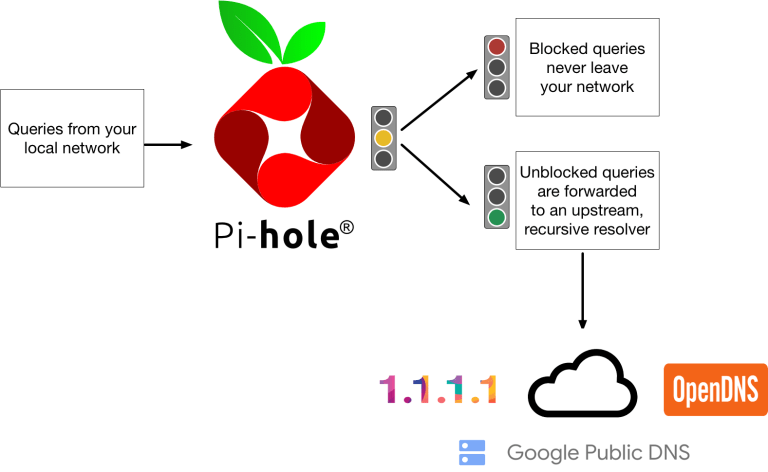
\includegraphics[width=1\textwidth]{Figures/pihole-dns}
\decoRule
\caption{The flow of traffic through the Pi-hole system}
\label{fig:circle}
\end{figure}

The flow of traffic goes like this:
\begin{enumerate}
\item The client asks the Pi-hole who is pi-hole.net
\item Pi-hole will check the cache and reply if the entry is present in the cache
\item Pi-hole will check the blocking list and if the domain is blocked, it will replay accordingly
\item If neither 2 or 3 are true, Pi-hole forwards the request to the external upstream DNS server, that was configured on installation
\item After receiving the answer from the upstream server, Pi-hole will reply to the client
\item Pi-hole save the answer in the cache to be able to respond more quickly if the same domain is queried again
\end{enumerate}

Pi-hole can also act as a network monitoring tool, since it logs all DNS queries sent to it, by default, so you can find what kind of traffic is going through your network. We integrated a component for visualizing this data into our system, to be able to quickly tell what domains are most visited by the children and what blocked domains they are trying to access. This integration was made easier by the fact that Pi-hole has a component which takes the raw data from the logs and pre-process it, storing it in a local database, to be able to serve quickly the types of queries needed, such as the top visited domains and the top blocked domains. We access this data by using a socket and some predefined commands. Pi-hole offers also a web interface to view these detailed reports. You can see the query types over time, forward destination over time, top domains, top blocked domains and other useful reports, as can be seen in the figure below.

\begin{figure}[th]
\centering
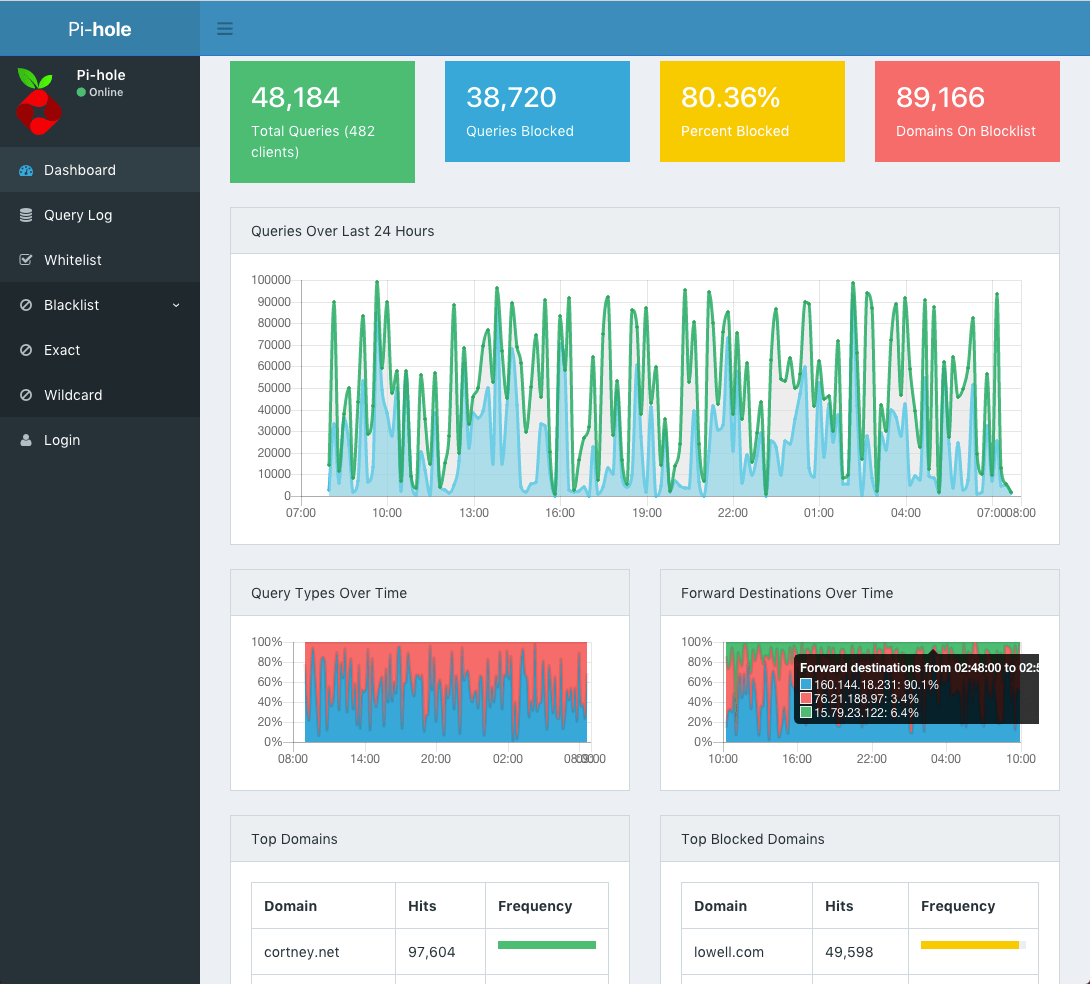
\includegraphics[width=1\textwidth]{Figures/pihole-admin}
\decoRule
\caption{The Pi-hole admin dashboard}
\label{fig:circle}
\end{figure}

Other benefits that Pi-hole brings to your local network are related to bandwidth and network speed. Because it works at the DNS level and prevents the ads and blocked domains from being downloaded. Since these ad images, videos and sounds are not being downloaded, the network will perform better. For the same reasons, it also reduces bandwidth, by preventing undesired assets from being downloaded. You can also extend the default block list to include sites that are known to serve malware or act as a phishing site, which brings another level of security, very important in the context of children using the Internet. The performance should not be a problem for the Pi-hole system, since even a not so powerful Raspberry Pi has been documented of handling up to 60 clients without problems, more than enough for a family network. \parencite{salmela20177things}

\section{Dnsmasq}

\section{Netfilter}

\section{Go Lang}

\section{Flutter}

\section{All together}

%----------------------------------------------------------------------------------------